\documentclass{standalone}
\usepackage[usenames,dvipsnames]{xcolor}
\usepackage{tikz}
\usetikzlibrary{arrows.meta, matrix}
\usetikzlibrary{decorations.pathreplacing}
\usepackage{pgfplots}


\begin{document}

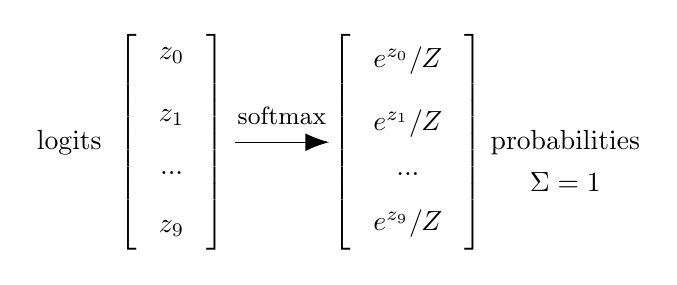
\begin{tikzpicture}

\matrix (m)[scale=3,matrix of math nodes,left delimiter={[},right delimiter={]}, column sep=5, row sep=10] at (0, 0)
{
z_0 \\
z_1 \\
... \\
z_9 \\
};

\draw [-{Latex[length=3mm]}] (0.8, 0) -- 
  node[above,shift={(0,	0.1)}] {\small softmax} 
(2,0);

\matrix (m)[scale=3,matrix of math nodes,left delimiter={[},right delimiter={]}, column sep=5, row sep=6] at (3, 0)
{
e^{z_0}/Z \\
e^{z_1}/Z \\
... \\
e^{z_9}/Z \\
};

\node[] at (-1.3,0) {logits};


% right brace
%\draw [decorate, decoration={brace, amplitude=10pt}] (4, 1.3) -- (4,-1.3);
% sum = 1
\node[] at (5,0) {probabilities};
\node[] at (5,-0.5) {$\Sigma = 1$};

\end{tikzpicture}

\end{document}